\documentclass[12pt,journal,compsoc]{D:/Магистратура/English/bare_conf/IEEEtran}
\newcommand\MYhyperrefoptions{
pdfpagemode={UseOutlines},plainpages=false,pdfpagelabels=true,
colorlinks=true,linkcolor={black},citecolor={black},urlcolor={black},
pdftitle={Working with attached to repair documents in the system of automatic registration of repairs},
pdfsubject={Typesetting},
pdfauthor={Arseny Zorin}}
\usepackage{graphicx}
\graphicspath{{D:/Магистратура/English/bare_conf/}}

\begin{document}
\title{Working with files attached to repair documents in the system of automatic registration of repairs}

\author{Arseny~Zorin}
\maketitle

\IEEEpeerreviewmaketitle



\section{Introduction}
\IEEEPARstart{S}ince the appearance of computers, progress hasn’t been  standing still. Technology has enormously improved in the last decade. Among trends that have appeared one can find a variety of wireless Internet accesses to printing prosthesis on 3D printers or cloud storages. The latter became storage de-facto standard in the past few years. It is used not only for private purposes, but also for corporates document storing and data archiving..

The object of the research is the authorized service center (ASC) located in St. Petersburg, Russia. ASC provides both warranty services and paid services of repair of household appliances. There are four ASC branches situated in different parts of the city. One can bring appliances for repair in to any of these four locations. During each repair operation performed by ASC a number of supporting attached documents is being generated  Each document has a title equal to a service ticket number::
\begin{itemize}
\item A photo of a schild from the backside of an appliance. This file is stored in a common folder for schilds photos by this manufacturer.
\item A scanned warranty ticket. This file is stored in a common folder for scanned documents by this manufacturer.
\item An outbound repair receipt. It is produced in cases when the repair was carried out at the client’s residence. This file is stored in a common folder of outbound repairs by this manufacturer.
\item Various acts provided to a client including a technical condition act, a non-repairable act, a replacing device act, etc. 
\end{itemize}

All document folders are stored at ASC offices and on the head office server. ASC data is transmitted between branches and the head office through FTP protocol.

This work was inspired by a need for modernization of tools for documents storage and transmission. The C\# software programming language was used in the practical part of the research  as an alternative to VBA. New libraries will be used for scanning documents and taking photo of the documents. All document storages were moved to the cloud. Data will be stored and treated at the distributed servers in network. One of the advantages of storing data in the cloud is that when using cloud storages, users have a possibility to access the data from different places and from different devices which have an Internet access. Also cloud storage can prevent losing information in case of failure of a local storage.

\section{Practical implementation}
\subsection{Working with AForge.NET}
\IEEEPARstart{T}aking photo of a schild: when the button is pressed, a new window with a video player element  opens. Stream video from selected web-camera will be played on this element. When the button "Take a snapshot" is pressed, there will be a capture of the picture from video player element and an obtained picture will be stored in the specified directory in .jpg format.

The .NET Framework does not support working with web-cameras. It means that there is no video playback element. However, there is namespace AForge.Controls with VideoSourcePlayer element in AForge.NET. This element was created only for being used in Windows Forms software. It’s been decided to use WPF for software development,and there are a few solution methods available:
\begin{itemize}
\item Creation of a hybrid application. In addition to the WPF window, there will be one Windows Forms window.
\item Using WindowsFormsHost element. This element allows to place Windows Forms element on WPF page.
\end{itemize}

The latter option  was selected. For its realization we have to add: System.Windows.Forms.Integration and AForge.Controls namespaces, WindowsFormsHost element and VideoSourcePlayer inside it. (Fig. 1)
\begin{figure}[h]
\centering
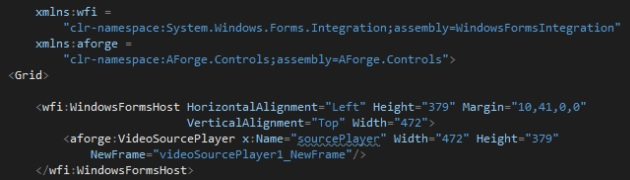
\includegraphics[width=0.5\textwidth]{1}
\centering
\caption{Adding namespces and elements}
\end{figure}

In addition to the playback element we have to add elements for interaction with VideoSourcePlayer element:
\begin{itemize}
\item "Take a snapshot" button
\item List of playback sources
\end{itemize}
After adding the above mentioned  elements, the window in "Constructor" mode will look like on fig. 2.
\begin{figure}[h]
\centering
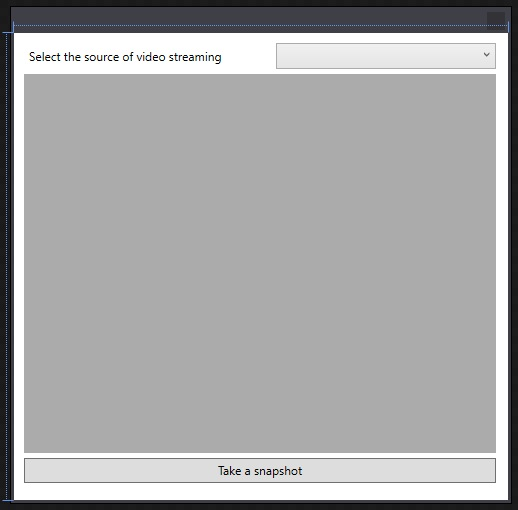
\includegraphics[width=0.5\textwidth]{2}
\centering
\caption{Window view in the constructor mode}
\end{figure}

There is AForge.Video.DirectShow. VideoCaptureDevice class for capturing video from an input-output (I/O) device. It is necessary to set device's moniker (the name of a specific instance of an object). It is a COM-object that has its own way to create and maintain a special interface - IMoniker), which will capture the picture. In addition, we have to add an event handler - NewFrame. Every time a new frame is received, this event will raise. The received frame is further sent to the handler in the Bitmap format. It can be processed and stored in the specified format in the right place.

The list will be filled with names of all connected I/O devices and the default device will be the first on the list.

The event comboBoxSources\_SelectedIndexChanged rises after changing selection of source. It stops streaming from previous I/O device, sets a moniker to the VideoCaptureDevice class of a new selected device and resumes streaming.

Pressing the button "Take a snapshot" changes the value of the take\_pict boolean variable onto true. The value of this variable checks in the event raised after receiving of a new frame. If its value equals to true, then the received image is saved in .jpg format in a dedicated place. In our case - Yandex.Disk.

The method EndOfWork, that stops streaming and frees used resources, is called after  closing the window.

\subsection{Working with TWAIN library}
\IEEEPARstart{W}e need to program a button for documents scanning. There will be displayed a selection of data sources after clicking on the button (if there are several connected scanners). When selecting of the source, scanning will start, and the received file will be stored in the specific folder in .jpeg format. We have to close data source after finishing the scanning.

There are a lot of different methods in the TWAIN library. However, only several of them will be used for completing the task:
\begin{itemize}
\item OpenDataSource() - Opens a data source. Type of return value - bool. Value true if operation is successful, else - false.
\item SelectDataSource() - Shows dialog window for selecting a data source. Type of return value - bool. Value true if operation is successful, else - false.
\item Property ShowUI - Gets or sets a value indicating whether to show user interface (UI) of TWAIN-source (to speed up value sets as false).
\item Acquire() - Gets an image from a data source. Type of return value - void.
\item GetImage(int index) - Returns a scanned image. The parameter index - index of return image. Type of return value - System.Drawing.Image.
\item CloseDataSource() - Closes a data source. Type of return value - bool. Value true if operation is successful, else - false.
\end{itemize}

The platform of developed software was changed to 32-bit(x86). The reason is that 64-bit(x64) platform is not supported with all scanners.

\subsection{Working with Microsoft.Office.Interop}
\IEEEPARstart{T}o begin working with Word and Excel documents from Visual Studio, it is necessary to add references into the project: Microsoft.Office.Interop.Word and Microsoft.Office.Interop.Excel.

\subsubsection{Working with Microsoft.Office.Interop.Word}
\IEEEPARstart{T}he words starting with \@ must be replaced with values of table cells during the creation of acts. Application object, which is the parent of all objects, is used for working in the .NET. We can work with its methods and properties when the reference on this object is received. This object provides a large set of methods and properties that allows to manage  Microsoft Word. In particularly, all Word functions require an object parameters.

There are two important moments in relation to working with Word through C\# that are worth noting:
\begin{itemize}
\item An unmanaged resource is created. It is a separate process stored in buffer memory within Word application. This process will not be collected with a garbage collector. If it is not closed and showed on the screen, it will remain in the computer memory until turning the computer off. Such processes are acсumulated invisibly for the user. The programmer must take care of closing the unmanaged resources.
\item Word runs invisible by default, we need to display it by ourselves.
\end{itemize}

Despite the latter fact, in our case, Word document will be invisible for the user. However, EndOfWork method will close this process.

Object Range - the main object for working with Word- is the region in the document that can include a pair of characters, tables, bookmarks etc. There is Selection object - part of document selected with pointer, that can be converted into the Range. For task execution we have to get Range for the whole document, then to find necessary string in received Range, get Range for this string and inside the latter Range to change the text on required.

There is a rare error in the Microsoft.Office.Interop library that was accepted by Microsoft company. The error is exiting Execute method from Find interface with "Stub received bad data" error. The reason is that we use Globally Unique Identifiers (GUIDs) in Word that were used in Excel 95. These identifiers begin to specify in Excel library if Excel 95 library was registered later than Word library. It causes  incorrect construction of proxy v-table for out-of-process clients. As a result, queries to that table causes an error or a failure, because instead of sending to the Word they are sending to the Excel.

Standard search and replacement of a string with Interop.Word.Find interface must be replaced with the library System.Reflection.

When a work with the template is over, it is being printed with standard method PrintOut. In some cases filled template must be saved. The question about saving a template will be prompted at the user.

\subsubsection{Working with Microsoft.Office.Interop.Excel}
\IEEEPARstart{W}ork with Excel through C\# is much easier than with Word. We are working with cells instead of Range.

Application object is also used for the work with Microsoft Excel through .NET. And important facts are the same. These are: an unmanaged resource is created and it is invisible by default. In our case, Excel application must be visible. Used resources must be released from the code. However, if a document was closed before releasing, it could be an exception which has to be handled in try-catch block.

Working with Excel is similar to working with two-dimensional array.

\subsection{Working with Yandex.Disk}
\IEEEPARstart{T}he most popular cloud storages were studied and after all a decision to use Yandex.Disk was made. However, according to the overview and comparison of different clouds, Google Drive or Dropbox were named as the most appropriate tools for business needs . Dropbox wasn’t  selected because of limited amount of free space (only 2Gb). An interaction with our software not only via API but via WebDAV protocol too was the reason for selecting Yandex.Disk.

To begin with, WebDAV API was selected for interaction. With APIs we can use a cloud storage as an ordinary file system. WebDAV API is compliant to the WebDAV protocol because of its API that is compatible with different libraries and clients. Also Yandex has SDK for different popular platforms, including mobile.

OAuth token has to be received to begin working with Yandex.Disk from software. OAuth is an authorization protocol. According to this protocol, a developer has to register his software at the OAuth Yandex Server and request for an access to the data. Access is either granted or denied by an authorized user. While using OAuth protocol, user does not enter his password in the software and that’s why a user account can not be hacked. Received token has to be sent in an Authorization header every time an API is used.

Object of DiskSdkClient class has to be created and subscribed to its methods because all calls of SDK are asynchronous. Asynchrony in SDK is used for providing correct parallel changing of a user interface state from a parallel background thread.

There are methods appropriate to the actions on Yandex.Disk implemented in the SDK. Only used methods are discussed further:
\begin{itemize}
\item GetListAsync - Requests for content of a directory (paginated list of content can be received with GetListPageAsync method)
\item GetItemInfoAsync - Requests for a file/folder properties
\item MakeDirectoryAsync - Creates a directory
\item RemoveAsync - Deletes a file/folder
\item UploadFileAsync - Uploads a file
\item DownloadFileAsync - Downloads a file
\end{itemize}

Received files and folders data are stored in the fields of DiskItemInfo class object:
\begin{itemize}
\item DisplayName - Name of a file/folder, which should be displayed on a user interface of the software (OriginalDisplayName contains name of a file in URL format).
\item FullPath - The path to a file/folder from the root directory of the user (OriginalFullPath contains encoded URL).
\item ContentType - MIME-type of a file.
\item LastModified - Date and time of the last file modification.
\item CreationTime - Uploading date and time of file on the cloud.
\item Etag - Etag header for a file (MD5-sum).
\item PublicUrl - External link on a published file/folder.
\item ContentLength - Size of a file/folder (bytes).
\item IsDirectory - Returns the value that shows whether this element is a directory.
\item IsPublished - Returns the value that shows whether this file/folder is published.
\end{itemize}

Several methods have to be implemented:
\begin{itemize}
\item Method which checks an element in the specified directory for existing.
\item Method which opens selected file. First, it has to be downloaded.
\end{itemize}

We discovered a drawback of the asynchronous method that is GetListAsync was found during creation of the method that checks an existence of a file. The background thread which fills a  list with elements located in the specific directory is not completed before it is being in use because of asynchronous execution.To avoid this drawback it is necessary to wait for the completion of filling the list. Awaiting for filling was implemented with delaying of execution the code with System.Threading.Thread.Sleep(200) method which delays the code by 0.2 seconds (Fig. 3).
\begin{figure}[h]
\centering
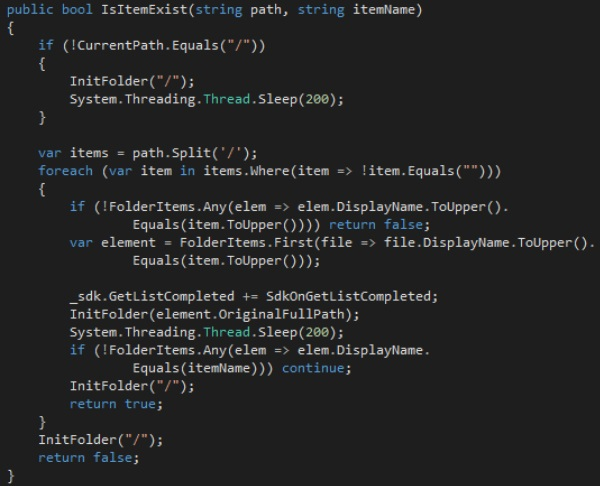
\includegraphics[width=0.5\textwidth]{3}
\centering
\caption{Pausse the thread}
\end{figure}

However, this solution of the problem is not correct because resourcing to this directory on another computer can take more time, in this case the list of elements will not be filled correct and it will lead to incorrect work of the whole method.

To fix this drawback in a right way,  it is necessary to change all the work performed by Yandex.Disk SDK. Thus, the decision was made to create the call to the cloud through WebDAV protocol and to liquidate an asynchrony. Since Class has not got any user interface, we can liquidate an asynchrony.

It is necessary to use WebDAV protocol methods to create an interaction with the cloud:
\begin{itemize}
\item PUT - Uploads a file
\item GET - Downloads a file
\item MKCOL - Creates a directory
\item COPY - Copiesa file/folder
\item MOVE - Move and renames a file/folder
\item DELETE - Deletes a file/folder
\item PROPFIND - Gets the properties of files/directories
\item PROPPATCH - Changes the properties of a file/directory

\end{itemize}

From the above listed methods we will need to use only 4 of them: PUT, GET, MKCOL and PROPFIND.

Classes HttpWebRequest and HttpWebResponse, which are included in the .NET Framework from version 2.0, will be used because WebDAV uses HTTP/S. Class HttpWebRequest represents HTTP-request, second - HTTP-response. Namespace System.Net for working with network has to be included. It is necessary to generate the request correctly in order for the WebDAV server to understand that.

Every method has its own parameters. Some of them are the same for all methods:
\begin{itemize}
\item Remote host address (https://webdav.yandex.ru/)
\item Authentication data. Yandex receives this data in two types: Basic - login and password; OAuth-token. For transmission thise data the string is used: request.Headers["Authorization"] = "OAuth " + AccessToken.
\item The command that has to be executed, e.g. request.Method="PUT"
\end{itemize}

The name of the directory, in which the method must be executed, is added to the address of the host in case of execution method in directory other than root.

Creation of a new directory in the cloud, i.e. execution MKCOL method, does not require any parameters except mandatory. WebDAV-protocol does not allow to create several subfolders in one request. If the directory already exists and request tries to create directory with the same name, then exception, that must be handled, rises. To find out whether the directory exist, we can send a request for creating the directory and handle the exception with code 405 - "Invalid method", which raises in case of creation the directory with the same name.

Requestion the properties -PROPFIND method, does not requires any parameters except mandatory too. However, it is necessary to parse received response (XML format) from the server. Besides parsing the response, it is necessary to catch an exception with 404 code - "Element not found".

Unlike other methods, PUT and GET requires for an additional parameters, like variables for data reading and writing.

For example, in addition to setting variables, for method GET to execute, we will need to get a file size from the header, create file stream for writing a file on a local drive, receive the stream from the server. The next step is reading the data from received stream and writing the data to the open stream. If the amount of read bytes are equal to read from the header, then file downloading is successful.

For method PUT it is necessary to set parameters:
 \begin{itemize}
\item AllowWriteStreamBuffering - It enables or disables data buffering before sending it. If it is enabled, then the file loads to the memory, first, and only after that to the server.
\item SendChunked - It allows to upload files of uncertain size to a remote host 
\item Expect100Continue - Parameter that includes waiting for a response from the server with code 100. It means that we can continue, in other casse its value will be false.
\end{itemize}

After completion formation of the query, it is necessary to receive a network flow where the data, which will be sent to the server, written in. We also need to open a local file for reading, allocate byte buffer for temporary storing data read from the file. Then read and send are produced in the cycle and data are written to the flow. Network and file flows are closed after that. HTTP status has to be checked for equality to the flag Created and to compared to the size of the file with amount of sended bytes. Sending is successful if both of this conditions are fulfilled, else - there was an error.

After synchronous methods were written, the decision was taken to compare the time of their execution with asynchronous. The Stopwatch class is used for the precise measurement of time. To an object of TimeSpan class the measured time is assigned after measurements were finished. Measurements are presented in a poped up window in hh:mm:ss.ms format (Fig. 4).
\begin{figure}[h]
\centering
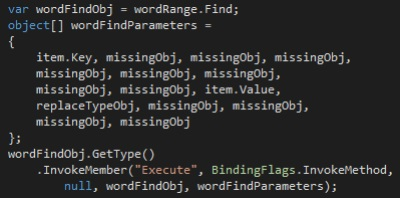
\includegraphics[width=0.5\textwidth]{4}
\centering
\caption{Measurement's results}
\end{figure}

According to the results, the best method for our targets is synchronous IsItemExist method.

Except downloading and uploading file to the server, it is necessary to organize the work with it. For example, the file has to be opened if it is an image. This method is realized in the OpenFile method, which downloads a file from the cloud and then opens it with LaunchFile method. We have to make sure that a user is finished working with it to delete a file, for this we show a window with a message. The file is closed and deleted if the window was closed.

\section{Conclusion}
\IEEEPARstart{A} software that allows user to take a snapshot of a document with a web-camera and a an attached file with a scanned copy generated with scanner was developed during execution of the practical part of the assignment. An ability to create different acts based on MS Word and MS Excel templates was organized. The work with files in the cloud was also organized.

Each task cold be solved with different ways. The choice of methods depends on  targets and programmer choice. For example, AForge.NET was selected for taking photos because of its simplicity and easy accessibility. TWAIN library, for working with scanner, was selected because of big amount of scanners that are TWAIN-devices. This library is time-tested and reliable besides a lot of TWAIN projects are on the Internet. Yandex.Disk was selected mostly because of the author’s personal experience.

The problem of lacking the video player WPF element was solved during the photo making task. For that, the WindowsHost element, that allows to include a Windows Forms element into WPF, was used.

The decision to move from 64-bit (x64) on 32-bit(x84) version of software was made, because of 64-bit version is not supported by all TWAIN-compatible scanners.

The work with templates was complicated because of with  an error that was accepted by Microsoft company. To avoid this error, the method, that in theory could be executed with one string, must be divided into three strings. This solution was suggested by Microsoft.

It was determined that the work with Yandex.Disk will not be an optimal due to its asynchronous nature. To  solve this defect, methods of appealing to the cloud server through WebDAV were created. At the end of the work measurements of execution synchronous and asynchronous methods were made. As it was shown in the results, in this case, synchronous methods are faster.

We can conclude that all tasks were fully solved. The goal of  software development as a subsystem for an ASC, that provides automation of tasks related to the attached documents, was achieved.
\end{document}
